% Created 2023-01-27 Fri 12:56
% Intended LaTeX compiler: pdflatex
\documentclass[letterpaper]{article}
\usepackage[utf8]{inputenc}
\usepackage[T1]{fontenc}
\usepackage{graphicx}
\usepackage{longtable}
\usepackage{wrapfig}
\usepackage{rotating}
\usepackage[normalem]{ulem}
\usepackage{amsmath}
\usepackage{amssymb}
\usepackage{capt-of}
\usepackage{hyperref}
\usepackage[margin=1in]{geometry}
\usepackage{placeins}
\usepackage{amsmath}
\usepackage{graphicx}
\usepackage{subcaption}
\usepackage{tikz}
\usepackage{upgreek}
\usepackage[separate-uncertainty=true, multi-part-units=single]{siunitx}
\tikzset{every picture/.style={line width=0.75pt}} %set default line width to 0.75pt
\usepackage{multicol}
\usepackage{setspace}
\usepackage{marvosym}
\setstretch{1.65}
\usepackage{centernot}
\usepackage{pifont}% http://ctan.org/pkg/pifont
\usepackage{tabularray}
\usepackage{svg}
\newcommand{\cmark}{\ding{51}}%
\newcommand{\xmark}{\ding{55}}%
\author{Duncan Britt}
\date{\today}
\title{Obstacle Avoidance\\\medskip
\large Case Analysis}
\hypersetup{
 pdfauthor={Duncan Britt},
 pdftitle={Obstacle Avoidance},
 pdfkeywords={},
 pdfsubject={},
 pdfcreator={Emacs 28.1 (Org mode 9.5.2)}, 
 pdflang={English}}
\begin{document}

\maketitle
The purpose of this document is to describe and contrast a couple of strategies for detecting obstacles, and to show their strengths and weaknesses by analyzing their performance in a variety of contexts.

\section*{Strategy \(A\)}
\label{sec:org42b97cc}
Strategy \(A\) aims to prevent any obstacles from entering the radial extent of the robot using a front facing distance sensor mounted on a servo, continuously sweeping side to side.

\begin{center}
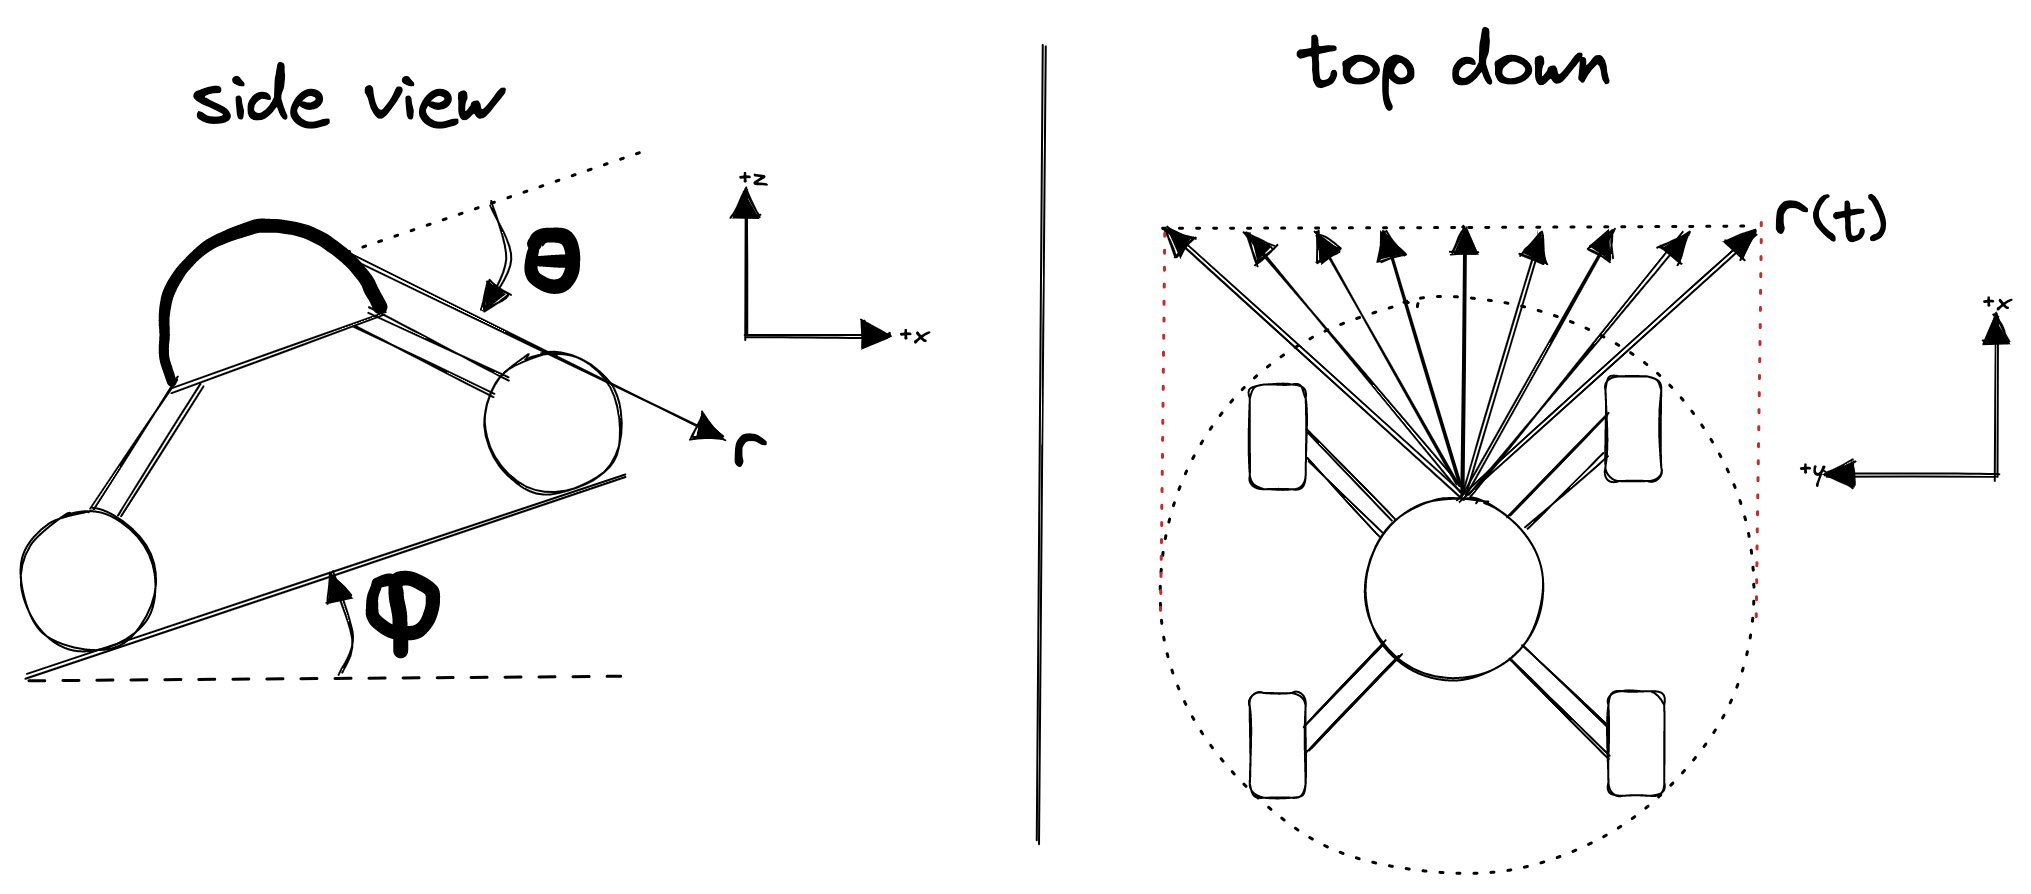
\includegraphics[width=.9\linewidth]{./strategy-a.png}
\end{center}

Let \(r\) be the reading from the distance sensor at time \(t\).
Let \(\upphi\) be the angle of inclination of the robot at time \(t\).
Let \(\uptheta\) be the maximum angle of inclination that we decide is safe for the robot.
The distance sensor would be aimed \(\uptheta\) degrees below the horizontal axis with respect to the robot.

\begin{center}
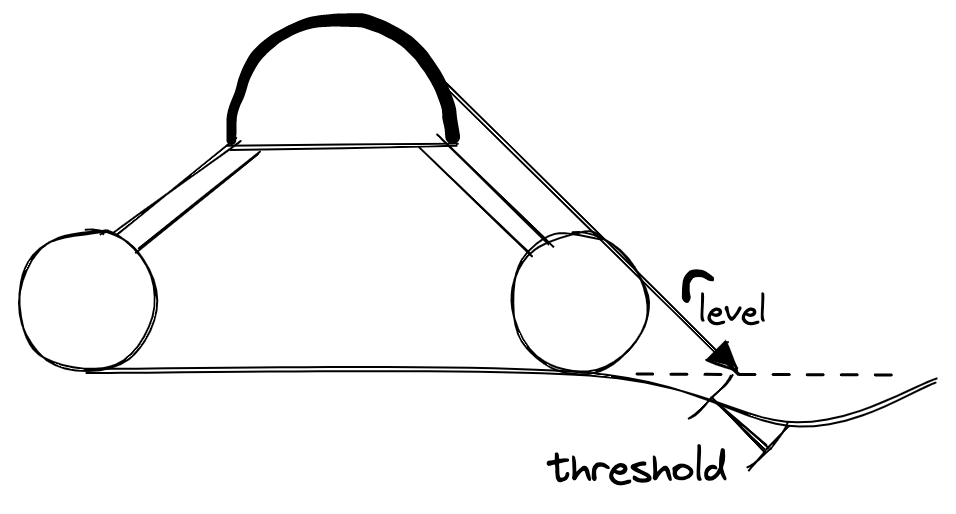
\includegraphics[width=300px]{./strategy-a2.png}
\end{center}

The robot would determine that there is an obstacle if
\begin{itemize}
\item the distance reading is sufficiently different from the distance reading that would be predicted by level ground, and
\item the rate of change in the distance reading is not small
\end{itemize}
\begin{align*}
A(r) = \left( \lvert r - r_{level} \rvert > \mathrm{threshold} \right) \land \left( \Delta r > \mathrm{threshold} \right)
\end{align*}
This strategy successfully handles cases 1-6 from the table below, but fails case 7.

\section*{Strategy \(A^{'}\)}
\label{sec:org0ba3cd9}
To overcome this, a slight modification to the previous strategy involves considering the robot's angle of inclination. If we assume that the terrain we will face in April will be sandy enough that there won't be holes on steep inclines, then we could decide that the extent to which we are concerned about holes is a function of the angle of inclination.

\begin{align*}
A^{'}(r) = & \left[ \left( r > r_{level} + \mathrm{threshold(\upphi)} \right) \land \left( \Delta r > \mathrm{threshold} \right) \right] \\
& \lor \left[ \left( r < r_{level} - \mathrm{threshold} \right) \land \left( \Delta r > \mathrm{threshold} \right) \right]
\end{align*}

\section*{Strategy \(B\)}
\label{sec:org64a08c5}
Strategy \(B\) does not attempt to prevent obstacles from entering the radial extend of the robot. It only attempts to prevent the robot from contacting obstacles.

\begin{center}
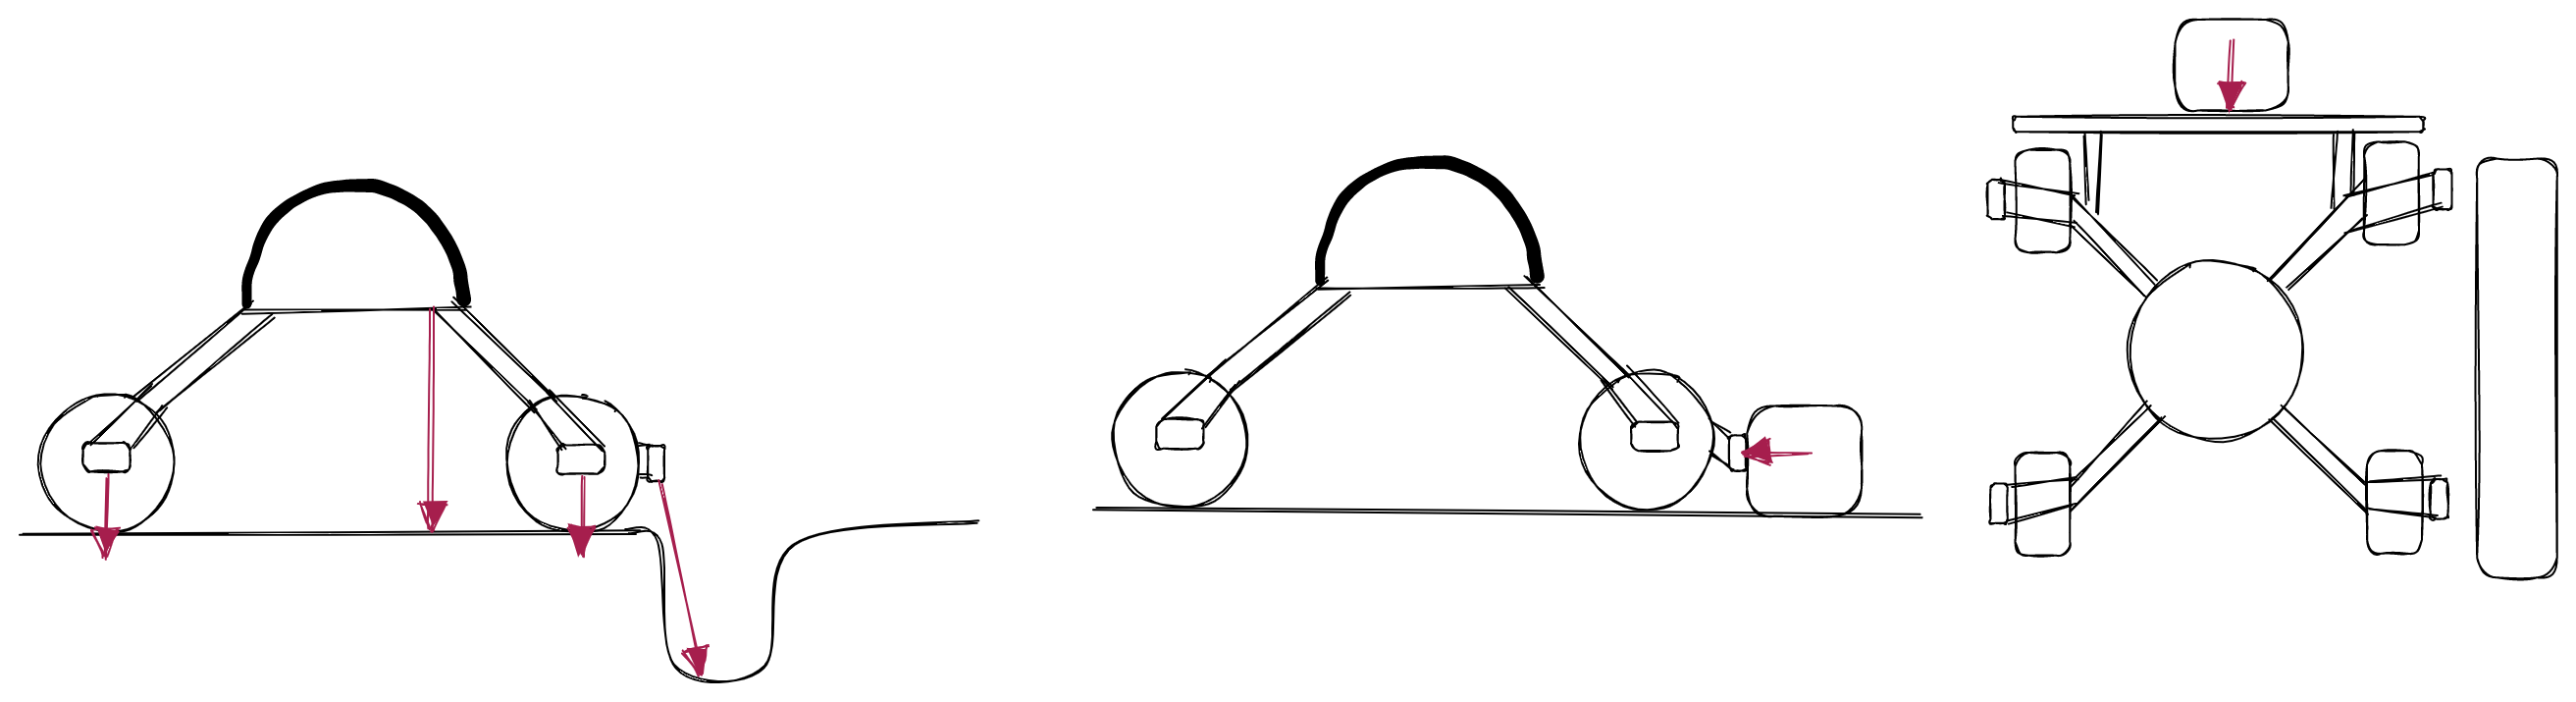
\includegraphics[width=.9\linewidth]{./strategy-b.png}
\end{center}

We would put infrared sensors facing down, or at a slight angle from the vertical axis, on the front and outer sides of the wheels, as well as on the underside of the middle of the chassis. These would be our hole detectors. We would also have a crossbar attached to a touch sensor on the front of the robot and touch sensors on the sides of the wheels.

We could then determine the presence of obstacles if they touch the front or sides of the robot, and we would find holes when we run into them.

\section*{Advantages \& Disadvantages}
\label{sec:orgdf991c9}

\(A\) is perhaps more complicated and difficult to get right. There's a lot of math involved. It also fails the case where the robot runs into grass. There's a concern that we might mistakenly detect a hole where none exists when coming over hills. \(A'\) tries to solve this, but it isn't obvious how successful the strategy will be. But, \(A\) and \(A^'\) have the advantage that they avoid obstacles entering the radial extend of the robot. This makes path planning much easier, as we would always know that we could turn \(360^{\circ}\) to face whichever direction we'd like to go.

\(B\) is more straightforward and handles more cases than \(A\), but has the disadvantage that it requires many more sensors and doesn't prevent obstacles from entering the radial extent of the robot. This makes path planning significantly harder.

A modification \(B^'\) could be to put a circular bar around the robot so that the touch sensor would detect obstacles on all sides and have infrared sensors below it. This could prevent obstacles from entering the radial extent of the robot and make path planning orders of magnitude easier.
\end{document}